\thispagestyle{empty}
\null
\vfill
\begin{center}
   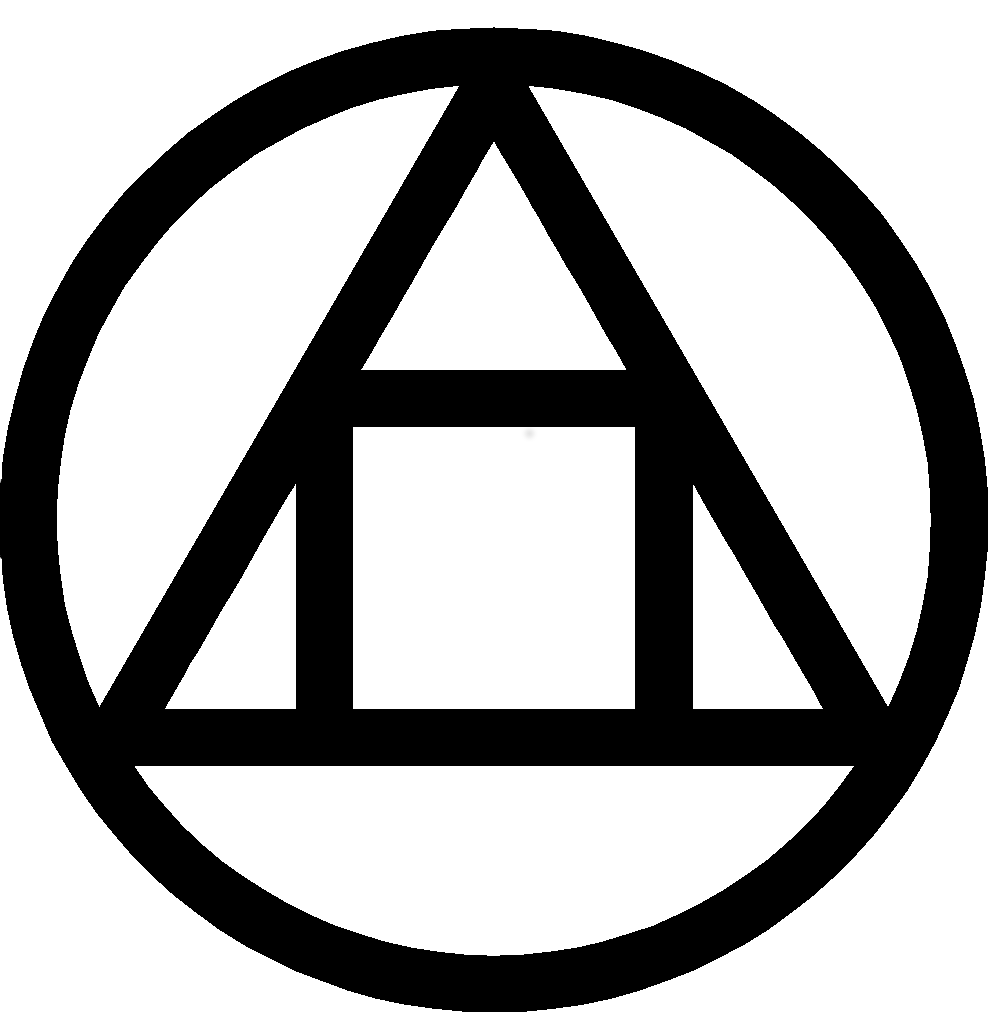
\includegraphics[width=0.9\textwidth]{res/sektionsvisor.png}
   \section{Sektionsvisor}
\end{center}
\vfill
\newpage

\subsection{Hyllningsvisa till Teknisk Fysik}
\textit{Mel: Sit on my face}\\
\index[alfa]{Hyllningsvisa till Teknisk Fysik}
\index[anfa]{Teknisk Fysik är mössbeklädda töntar...}
\begin{parse lines}[\noindent]{#1\\}

Teknisk Fysik är mössbeklädda töntar
fula flickor och en samling mammas pojkar.
Liknar mest en televerksbil,
som gått för många mil
En teknisk fossil!

Teknisk Fysik är lättare än att fjärta
Döda älgar värmer nu mitt kalla hjärta
Ta hit dynamit, sprängteknik, vårt gebit
Dessa tofsprydda avskum som ger oss kolik!
Dessa tofsprydda avskum som ger oss kolik!
Dessa tofsprydda avskum som ger oss kolik!
Dessa tekniska lik! Barambam!
\end{parse lines}
\vfill
\noindent
\textit{Skrevs av V-sektionen till en Sångarstrid, men stals lumpet av
F-sektionen som framförde den innan V fick chansen.}

\subsection{Everywhere we go}
\textit{Mel: Everywhere we go}\\
\index[alfa]{Everywhere we go}
\index[anfa]{Everywhere we go...}
\begin{parse lines}[\noindent]{#1\\}

Everywhere we go
People wanna know
Who we are
So we tell them

We are the E-sek
Mighty, mighty E-sek

$\vert\vert$: Uh, ah, oh E-sek :$\vert\vert$ (3 ggr)
\end{parse lines}

\subsection{Vår färg är röd}
\textit{Mel: When the saints go marching in}\\
\index[alfa]{Vår färg är röd}
\index[anfa]{Vår färg är röd}
\begin{parse lines}[\noindent]{#1\\}

Vår färg är röd, vår färg är fin,
för det är vi som går Maskin
Och vi har kommit för att dricka alkohol,
för det är vi som går Maskin
\end{parse lines}

\newpage
\subsection{Brand, Lant, Väg och Vatten}
\textit{Mel: Högst vinner}\\
\index[alfa]{Brand, Lant, Väg och Vatten}
\index[anfa]{Brand, Lant, Väg och Vatten...}
\begin{parse lines}[\noindent]{#1\\}

Brand, Lant, Väg och Vatten,
Störst på LTH
Ingenting kan stoppa oss,
V-sek allez allez
\end{parse lines}


\subsection{A-sek är bäst}
\textit{Mel: Rule Britannia}\\
\index[alfa]{A-sek är bäst}
\index[anfa]{A-sektionen den skiner såsom solen...}
\begin{parse lines}[\noindent]{#1\\}

A-sektionen den skiner såsom solen.
A-sek är grym på fest, ja A-sek är bäst!
\end{parse lines}



\newpage
\subsection{Kemisternas kampvisa}
\textit{Mel: Eslövs nationalsång}\\
\index[alfa]{Kemisternas kampvisa}
\index[anfa]{Vi är kemister och vi älskar maskinister...}
\begin{parse lines}[\noindent]{#1\\}

Vi är kemister och vi älskar maskinister
Vi är kemister och vi pussar arkitekt
Vi är kemister och vi kramar väg och vatten
Vi är kemister och vi är allra bäst!

Å.. spela, spela data!
Å.. heja, heja F!
Å.. koppla in elektro!
Å.. men K är allra bäst!
\end{parse lines}


\subsection{ING från sundets pärla}
\textit{Mel: Whistle stop (från Robin Hood)}\\
\index[alfa]{ING från sundets pärla}
\index[anfa]{För vi är ING från sundets pärla...}
\begin{parse lines}[\noindent]{#1\\}

För vi är ING från sundets pärla,
och det är fest idag igen,
och vi ska supa hela natten lång
och sjunga denna sång!

Raj-di-daj-daj-daj…
\end{parse lines}

\newpage
\subsection{Turkosa samban}
\textit{Mel: Samba de Janeriro }\\
\index[alfa]{Turkosa samban}
\index[anfa]{SAMBA"! Turkos turkos, här gör vi entré...}
\begin{parse lines}[\noindent]{#1\\}

SAMBA!

Turkos turkos, här gör vi entré
Vi bränner sprit uti KC:G
Turkos turkos, så gör dubbel-W
Mitt glas är två för att jag är sne!

$\vert\vert$: Simma sí, ah simma,
ah simma simma simma :$\vert\vert$ (4ggr)
\end{parse lines}


\subsection{Bortom vägar och vatten}
\textit{Mel: Pomp and Circumstance}\\
\index[alfa]{Bortom vägar och vatten}
\index[anfa]{Bortom vägar och vatten...}
\begin{parse lines}[\noindent]{#1\\}

Bortom vägar och vatten,
långt långt över Maskin
innan Brand hunnit släckas,
blickar vi ner på Kemi.
Bam bam bam!
Stolta står vi och väntar,
tills Elektro gjort sin sorti,
för vi är bästa sektionen,
och vi älskar vårat I!
\end{parse lines}

\newpage
\thispagestyle{empty}
\null
\vfill
\begin{center}

   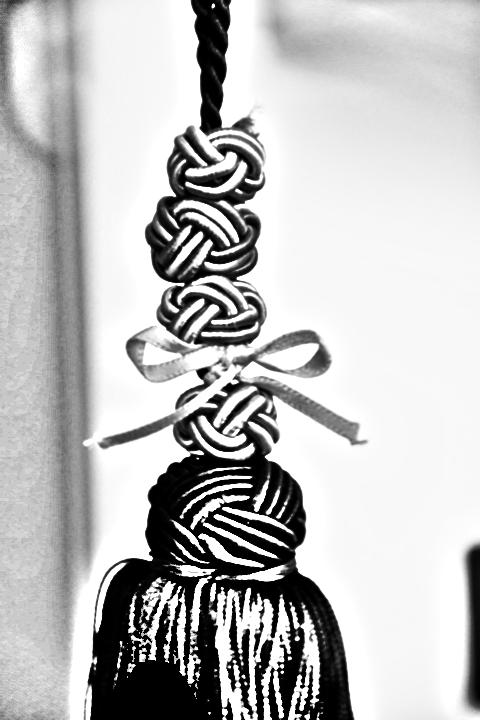
\includegraphics[width=0.8\textwidth]{res/dchip.jpg}
   \section{D-Chip}

\end{center}
\vfill
\newpage



\subsection{D-Chip är grymt}
\textit{Mel: Havet är djupt}\\
\index[alfa]{D-Chip är grymt}
\index[anfa]{De tror att det inte finns nå-...}
\begin{parse lines}[\noindent]{#1\\}

De tror att det inte finns nå-
gra tjejer på vår sektion.
Att vi bara dricker lättöl,
vad e det för slags fason?
Nej se dig omkring på dsek,
här finns vi och lustigt e
du kan inte bli besviken
det ska du snart få se!

att

D-Chip är grymt
D-Chip är grymt
Utanför källarn
är vi rätt sällan
men nu har vi rymt (alt. här får ni en skymt)

Å ganska råsa är vi här
så sjung nu så högt som rösten bär
för datatjejer
här har ni grejer
D-Chip är grymt!
\end{parse lines}


\subsection{Vill du koda med mig?}
\textit{Mel: Om sanningen ska fram}\\
\index[alfa]{Vill du koda med mig?}
\index[anfa]{Om jag lär mig alla namnen...}
\begin{parse lines}[\noindent]{#1\\}

Om jag lär mig alla namnen,
och Spritbolagets svans,
Om jag lär mig nollevisan,
skyddar chepsen med mitt liv.

Om jag köper mig en ouvve,
syr märken som en Gud.
Om jag respekterar staben,
lär mig våran nolledans.

$\vert\vert$: Vill du koda med mig då? Om sanningen ska fram?
Vill du koda med mig då? Vill du koda med mig? :$\vert\vert$

Om jag lär mig dricka minttu,
fast det faktiskt smakar skit.
Spöar phaddrarna på beer pong,
sätter trick shotsen från taket.

Och som alla phaddrar säger:
``Ingen hets, men det blir kul,
och det kommer säljas dricka
hashtag omduvill''

$\vert\vert$: Vill du koda med mig då? Om sanningen ska fram?
Vill du koda med mig då? Vill du koda med mig? :$\vert\vert$
\end{parse lines}


\subsection{Microchipvisa 2000}
\textit{Mel: Fångad av en stormvind}\\
\index[alfa]{Microchipvisa 2000}
\index[anfa]{Det folk inte kan förstå...}
\begin{parse lines}[\noindent]{#1\\}

Det folk inte kan förstå
Är kärleken som finns över Internet
Mina vänner undrar så
varför hjärtat bultar hårt när jag loggar in igen
Känslan när jag ser ditt namn på min skärm
pulsen ökar och jag blir alldeles varm

Jag är fångad med ett bredband, föll för dig,
när du skrev ett mejl till mig
du finns lagrad i mitt hjärta
Fångad med ett bredband, natt och dag
sitter jag här ensam kvar,
och väntar på din bild som laddas ner.

Jag borde ge mig av
för tiden går så fort i en datasal
Men min känsla stannar kvar
det är något som jag skulle ha förstått.
Jag vänder om igen och ser mig nu omkring
mejlen kommer ju från datorn bredvid mig.

Jag är fångad av en D-grabb, dig förstås.
Ingen alls kan hindra oss,
nu när skolan ligger öde.
Jag har fått en jackpot, här hos mig,
nu ska jag förföra dig,
i det ljus som skärmen strålar ut.

Vi surfar långsamt
uppkopplad på kärlekens band
Min längtan vaknar
när du ler
på väg mot cyberland
\end{parse lines}

\newpage
\null
\newpage
